% Earlier analysis of the original budgeted system (moved from the main paper).
\subsection{Setting and Method}
\textbf{Budgeted mapping.}
Let $G_t = \{g_1, \dots, g_N\}$ be the active map, $g_i = (\mu_i, \Sigma_i, \alpha_i, c_i)$, with streaming observation $(I_t, D_t)$ and pose $T_t$.
Per frame, a scheduler chooses a subset $A_t \subseteq G_t$ to optimize,
\begin{equation}
\max_{A_t \subseteq G_t} \Delta Q(A_t) \quad \text{s.t.} \quad \sum_{i \in A_t} C_i \le B_t,
\end{equation}
where $\Delta Q$ is the reconstruction improvement, approximated at runtime by a selector score, and $C_i(K) = C_i^{\mathrm{base}} + K \cdot C_i^{\mathrm{step}}$ is a decoupled cost model for $K$ microsteps.
The budget $B_t$ is \emph{modeled} optimization time.
\textbf{Measuring dilution.}
We log two age-resolved statistics per frame: the \emph{young budget share}, the fraction of modeled update budget spent on Gaussians younger than ten frames, and the \emph{mature selection rate}, the fraction of Gaussians at least ten frames old that are selected.
Dilution predicts a falling mature selection rate as the map grows.
\textbf{Selection.}
Candidates are scored by error $\times$ influence mass, optionally with temporal EMA filtering ($\beta = 0.90$), and packed by fractional-knapsack value density $s_i / C_i$ under $B_t = 15\,\mathrm{ms}$ with safety factor $1.10$ (effective cap $13.6\,\mathrm{ms}$).
Each selected Gaussian receives $K = 5$ microsteps; the cost model is calibrated so modeled and wall-clock optimization time agree within measurement noise on the RTX 4050 backend.
Exact Gaussian-to-pixel attribution costs $523.9\,\mathrm{ms}$/frame, so we use a center-sampled projection, $\tilde{m}_i = \alpha_i \det(\Sigma_{2D,i})^{1/4}\, e(\lfloor \mu_{2D,i} \rceil)$, that runs in $0.85\,\mathrm{ms}$ ($614.5\times$ faster) at Spearman $\rho = 0.9079$ and Pearson $r = 0.9028$ against exact attribution. The scheduler totals $2.54\,\mathrm{ms}$ per frame.
\textbf{Coverage throttling.}
Coverage $\kappa_t$ is the fraction of valid pixels with transmission $< 0.5$.
The per-frame spawn cap ramps from $1.0$ to $0.20$ as $\kappa_t$ goes from $0.80$ to $0.90$.
A backlog limit exists but was inactive in the headline runs, because its count was only computed when warmup was enabled; the factorial evaluates it independently.
Warmup pre-allocation is disabled and microsteps are fixed at $K = 5$.


\subsection{Diagnosing Compute Dilution}
\label{sec:oldexperiments}
\textbf{Protocol.} TUM RGB-D~\cite{sturm2012benchmark} and Replica~\cite{straub2019replica} sequences at $320 \times 240$, $B_t = 15\,\mathrm{ms}$, seeds $[42..49]$; two-sided paired Wilcoxon tests, Holm correction and bootstrap CIs over per-seed trajectory summaries; production \texttt{gsplat} backend; ground-truth poses with tracking decoupled (a mapping benchmark, not SLAM ATE).
With eight seeds the smallest attainable two-sided Wilcoxon $p$ is $0.0078$, and with fixed trajectories seeds measure repeatability only, so we report effect sizes with intervals and do not treat seed-level standardized effects as evidence of generalization.
Sequences use the first 150 frames where available; the local Replica copies provide 99 evaluated frames for \texttt{office0} and 119 for \texttt{office1}. All results in Tabs.~\ref{tab:main}--\ref{tab:method} come from one code revision (git tag \texttt{paper-rerun-1}) with the corrected evaluator: standard Gaussian-window SSIM and alpha-normalized rendered depth. Earlier bundles used a global-statistics SSIM and a depth evaluator that biased depth L1 toward zero in partially transparent pixels, so their SSIM and depth values are not comparable with these. Artifacts: \texttt{results/rerun\_paper1/}.
\textbf{Holdout protocol.} Because online mapping optimizes on the evaluated trajectory, train-view PSNR overstates generalization. We hold out every 8th frame render-only (never mapped, never selected) and report held-out effects in Tab.~S10. This is a same-trajectory proxy, not independent novel-trajectory generalization.

\begin{table*}[t]
\centering
\small
\begin{tabular}{lcccccc}
\toprule
\textbf{Policy} & \textbf{Mean PSNR} & \textbf{Final PSNR} & \textbf{SSIM} & \textbf{FPS} & \textbf{Map} & \textbf{$\Delta$ vs OURS} \\
\midrule
\texttt{no\_op} & 18.85 & 14.75 & 0.4655 & 67.2 & 21,128 & +8.89 $\checkmark$ \\
\texttt{error\_only} & 24.21 & 20.20 & 0.7023 & 11.0 & 72,366 & +3.53 $\checkmark$ \\
\texttt{error\_influence} & 25.38 & 22.35 & 0.7338 & 11.1 & 86,988 & +2.36 $\checkmark$ \\
\texttt{error\_influence\_temporal} & 25.23 & 22.05 & 0.7315 & 10.9 & 86,187 & +2.51 $\checkmark$ \\
\texttt{rtg\_slam\_reimpl} & 23.53 & 20.57 & 0.6833 & 10.1 & 60,050 & +4.21 $\checkmark$ \\
\textbf{OURS} & \textbf{27.74} & \textbf{28.73} & \textbf{0.7978} & \textbf{12.1} & \textbf{21,642} & --- \\
\textit{FULL} & \textit{27.89} & \textit{29.29} & \textit{0.8036} & \textit{11.3} & \textit{70,295} & -0.15 $\checkmark$ \\
\bottomrule
\end{tabular}
\caption{\textbf{Main benchmark, TUM \texttt{fr2\_xyz}, 150 frames $\times$ 8 seeds.} All six controls differ significantly from OURS after Holm correction ($p_{\mathrm{Holm}} = 0.0469$). FULL is $0.15\,\mathrm{dB}$ higher. Headroom recovery is $98.3\%$ relative to no-op and $94.0\%$ relative to the strongest budgeted baseline, at a $3.2\times$ smaller map than FULL. Source: commit tag \texttt{paper-rerun-1}.}
\label{tab:main}
\end{table*}


\begin{table*}[t]
\centering
\footnotesize\setlength{\tabcolsep}{4pt}
\begin{tabular}{lcccccc}
\toprule
& \multicolumn{3}{c}{TUM \texttt{fr2\_xyz}} & \multicolumn{3}{c}{TUM \texttt{fr1\_xyz}} \\
\textbf{Selector / map control} & \textbf{PSNR} & \textbf{Depth L1} & \textbf{Map (k)} & \textbf{PSNR} & \textbf{Depth L1} & \textbf{Map (k)} \\
\midrule
Error, no throttle & 24.13 & .0205 & 73.1 & 21.52 & .0378 & 79.1 \\
Error, coverage & 27.66 & .0118 & 21.7 & 23.23 & .0335 & 37.1 \\
Error, coverage + backlog & 27.67 & .0117 & 21.5 & 23.32 & .0334 & 35.1 \\
Temporal$\times$influence, no throttle & 25.26 & .0134 & 86.2 & 22.28 & .0368 & 85.5 \\
Temporal$\times$influence, coverage & 27.75 & .0108 & 21.5 & 23.78 & .0314 & 37.9 \\
Temporal$\times$influence, coverage + backlog & 27.73 & .0109 & 21.8 & 23.89 & .0318 & 33.1 \\
\midrule
Error, optimization budget $\times4$ & 27.82 & .0107 & 71.3 & 24.46 & .0309 & 79.1 \\
Error, hard map cap 23k & 26.89 & .0217 & 23.0 & 22.52 & .1075 & 23.0 \\
Error, hard map cap 39k & 24.93 & .0237 & 39.0 & 21.56 & .1029 & 39.0 \\
\bottomrule
\end{tabular}
\caption{\textbf{Corrected-pose factorial and dilution controls, 150 frames $\times$ 8 seeds per scene.} All factorial cells use the same modeled $15\,\mathrm{ms}$ optimization budget. The $\times4$ control uses $60\,\mathrm{ms}$ for optimization while keeping the original $15\,\mathrm{ms}$ spawn allowance. Depth L1 is in meters. Backlog is enabled independently of warmup only in the last throttle level. Per-run traces and paired intervals are in \texttt{results/rerun\_paper1/dilution\_factorial/}.}
\label{tab:factorial}
\end{table*}


\textbf{Main result (Tab.~\ref{tab:main}; Supp.\ Figs.~S4--S5).}
OURS reaches $27.74 \pm 0.03\,\mathrm{dB}$: $+2.36$ over the strongest budgeted baseline, $+4.21$ over the RTG-SLAM-policy re-implementation, and $+8.89$ over pass-through. These results evaluate the combined policy on this trajectory.

\textbf{Selector $\times$ throttle factorial (Tab.~\ref{tab:factorial}).}
With selector fixed to raw error, coverage adds $+3.53$ $[3.38,3.70]$ dB on \texttt{fr2\_xyz} and $+1.71$ $[1.64,1.80]$ dB on \texttt{fr1\_xyz}. With temporal$\times$influence fixed, its gains are $+2.49$ $[2.40,2.59]$ and $+1.50$ $[1.48,1.52]$ dB. Brackets are paired seed-bootstrap 95\% CIs; all four coverage contrasts have two-sided paired Wilcoxon $p=.0078$. Temporal selection itself adds $+0.09$ dB with coverage on \texttt{fr2\_xyz} and $+0.54$ dB on \texttt{fr1\_xyz}; the interaction is negative ($-1.04$ and $-0.22$ dB), so selector and coverage effects are not additive. The independent backlog option adds $+0.01$/$-0.02$ dB on \texttt{fr2\_xyz} and $+0.08$/$+0.11$ dB on \texttt{fr1\_xyz} for error/temporal selection.

\textbf{Dilution controls and direct allocation.}
Holding the spawn allowance at its $15\,\mathrm{ms}$ value, giving raw-error selection $60\,\mathrm{ms}$ for optimization raises PSNR by $+3.69$ $[3.55,3.83]$ and $+2.94$ $[2.89,3.01]$ dB on \texttt{fr2\_xyz}/\texttt{fr1\_xyz}, despite maps of $71\mathrm{k}$/$79\mathrm{k}$. Capping the error-only map at 23k adds $+2.76$ $[2.62,2.90]$ and $+1.00$ $[0.96,1.05]$ dB, but multiplies depth L1 by $2.8$ on \texttt{fr1\_xyz}. A 39k cap, close to that scene's coverage map size, adds $+0.04$ $[-0.03,0.10]$ dB there (and $+0.80$ $[0.67,0.93]$ dB on \texttt{fr2\_xyz}). Thus a static size limit does not reproduce coverage throttling's effect on \texttt{fr1\_xyz}. For raw-error selection on \texttt{fr2\_xyz}, coverage reduces the share of modeled update budget spent on Gaussians younger than ten frames from $22.7\%$ to $9.5\%$, while the per-frame selection rate among mature Gaussians rises from $37.9\%$ to $87.4\%$. The corresponding mature selection rate on \texttt{fr1\_xyz} rises from $28.8\%$ to $57.4\%$. Allocation shifts and the budget intervention support compute dilution under the tested protocol, but coverage throttling also changes the optimization trajectory (its spawn cap carries most of the effect; see the decomposition below). Map size alone is not identified as the unique cause.



\begin{figure*}[tbp]
\centering
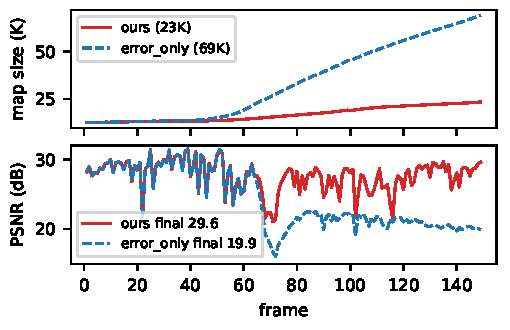
\includegraphics[width=0.92\textwidth]{figs/fig7_dilution.pdf}
\caption{\textbf{Map growth and reconstruction quality over time} on TUM \texttt{fr2\_xyz} and \texttt{fr1\_xyz} (150 frames, eight seeds). Lines show the seed mean and shaded bands show $\pm1$ standard deviation. \texttt{error\_only} versus \texttt{error + coverage} holds the selector fixed to show the coverage effect; \texttt{temporal + coverage} adds the combined policy. Paired sequence-level contrasts are reported in Tab.~\ref{tab:factorial}.}
\label{fig:dilution}
\end{figure*}

\textbf{Replica factorial and proportional budget (Tab.~\ref{tab:replica}).}
We ran the same selector$\times$throttle cells on two Replica scenes. Unlike TUM, coverage throttling lowers raw-error PSNR ($-0.68$ and $-0.87$ dB on \texttt{office0} and \texttt{office1}) and shrinks the map ($113$k to $65$k and $84$k to $40$k); backlog throttling is worse still ($-2.55$ and $-2.04$ dB relative to coverage alone, with depth L1 up by $0.12$ and $0.05$\,m). Without throttling, the temporal-influence selector trails raw error by $1.95$ and $2.33$ dB. Budget interventions help: a fixed $\times4$ budget adds $+2.81$ and $+1.56$ dB, and a budget proportional to map size (mean scale $3.67\times$ and $3.87\times$, map size unchanged) adds $+2.88$ and $+1.56$ dB. On TUM the proportional budget adds $+3.73$ and $+2.99$ dB on \texttt{fr2\_xyz} and \texttt{fr1\_xyz} over the unthrottled baseline measured in the same batch ($24.16$ and $21.54$ dB). These batches use the same code revision as Tabs.~\ref{tab:main} and~\ref{tab:factorial}.
\begin{table*}[t]
\centering
\footnotesize\setlength{\tabcolsep}{4pt}
\begin{tabular}{lcccccc}
\toprule
& \multicolumn{3}{c}{Replica \texttt{office0}} & \multicolumn{3}{c}{Replica \texttt{office1}} \\
\textbf{Condition} & \textbf{PSNR} & \textbf{Depth L1} & \textbf{Map (k)} & \textbf{PSNR} & \textbf{Depth L1} & \textbf{Map (k)} \\
\midrule
Error, no throttle & 30.63 & .0403 & 112.7 & 33.84 & .0161 & 84.2 \\
Error, coverage & 29.95 & .0556 & 65.2 & 32.97 & .0273 & 39.9 \\
Error, coverage + backlog & 27.40 & .1720 & 45.7 & 30.93 & .0744 & 25.9 \\
Temporal$\times$influence, no throttle & 28.68 & .0489 & 115.8 & 31.51 & .0202 & 85.8 \\
Temporal$\times$influence, coverage & 28.14 & .0651 & 66.3 & 31.73 & .0329 & 42.0 \\
Temporal$\times$influence, coverage + backlog & 26.18 & .2385 & 45.8 & 29.79 & .1093 & 24.1 \\
\midrule
Error, optimization budget $\times4$ & 33.44 & .0326 & 107.5 & 35.41 & .0106 & 82.8 \\
Error, budget $\propto$ map size & 33.51 & .0327 & 107.5 & 35.41 & .0108 & 82.7 \\
\bottomrule
\end{tabular}
\caption{\textbf{Replica factorial and map-proportional budget, 99 (\texttt{office0}) and 119 (\texttt{office1}) frames $\times$ 8 seeds per scene.} Same cells as Tab.~\ref{tab:factorial}; all runs use the current code revision and a $15\,\mathrm{ms}$ modeled budget unless stated. The proportional cell sets the optimization budget to $15\,\mathrm{ms}\times N_t/N_{\mathrm{ref}}$ (mean scale $3.7$--$3.9\times$) with the spawn allowance fixed at $15\,\mathrm{ms}$. Coverage and backlog throttling lower PSNR on Replica, whereas more optimization budget raises it.}
\label{tab:replica}
\end{table*}


\textbf{Scene-level evidence (Tab.~\ref{tab:scenelevel}).}
Because the unit of generalization is the scene, we ran the unthrottled, coverage-throttled and map-proportional raw-error policies on 11 further scenes (six Replica, five TUM; 99 frames, three seeds) and pooled them with the four scenes above. The map-proportional budget improves PSNR on all 15 scenes (median $+2.70$ dB, range $+0.02$ to $+3.73$ dB; exact sign test $p<10^{-4}$); the one near-zero gain is the small-map static scene \texttt{fr3\_sitting\_static} ($+0.02$ dB, $17$k Gaussians). Coverage throttling improves PSNR on 5 of 15 scenes (median $-0.13$ dB, range $-1.64$ to $+3.53$ dB; sign test $p=0.30$). The proportional-budget gain tends to grow with the unthrottled map size (Spearman $+0.52$, $p=0.048$, $n=15$, exploratory), as dilution predicts. Per-scene intervals are over three or eight seeds on a fixed trajectory, so the sign and scale across scenes are the evidence. More budget helps any compute-limited optimizer: this shows that raw-error selection under a $15\,\mathrm{ms}$ budget is compute limited in every scene tested, not that growth is the cause.
\begin{table*}[t]
\centering
\footnotesize\setlength{\tabcolsep}{4pt}
\begin{tabular}{lccclccc}
\toprule
\textbf{Scene} & \textbf{Prop.} & \textbf{Cov.} & \textbf{Map (k)} & \textbf{Scene} & \textbf{Prop.} & \textbf{Cov.} & \textbf{Map (k)} \\
\midrule
\texttt{fr2\_xyz} (T) & +3.73 & +3.53 & 75 & \texttt{office1} (R) & +1.56 & $-$0.87 & 84 \\
\texttt{fr1\_xyz} (T) & +2.99 & +1.71 & 79 & \texttt{office2} (R) & +2.76 & $-$0.08 & 115 \\
\texttt{fr1\_desk} (T) & +0.92 & $-$0.16 & 60 & \texttt{office3} (R) & +3.55 & $-$0.26 & 148 \\
\texttt{fr1\_room} (T) & +1.74 & $-$0.13 & 103 & \texttt{office4} (R) & +3.68 & $-$0.04 & 135 \\
\texttt{fr1\_rpy} (T) & +2.06 & +0.04 & 72 & \texttt{room0} (R) & +2.54 & $-$0.19 & 149 \\
\texttt{fr3\_sitting\_static} (T) & +0.02 & +0.08 & 17 & \texttt{room1} (R) & +2.12 & $-$0.25 & 102 \\
\texttt{fr3\_structure\_texture\_near} (T) & +2.70 & +2.54 & 61 & \texttt{room2} (R) & +3.09 & $-$1.64 & 145 \\
\texttt{office0} (R) & +2.88 & $-$0.68 & 113 &  & & &  \\
\bottomrule
\end{tabular}
\caption{\textbf{Scene-level change in mean PSNR (dB) relative to unthrottled raw-error selection, 15 scenes.} Prop.: optimization budget proportional to map size; Cov.: coverage throttling; Map: final size of the unthrottled map. T: TUM, R: Replica. \texttt{fr2\_xyz}, \texttt{fr1\_xyz}, \texttt{office0} and \texttt{office1} use 150 frames and eight seeds; the others use 99 frames and three seeds. Proportional budget is positive on 15 of 15 scenes (median $+2.70$, exact sign test $p<10^{-4}$); coverage throttling on 5 of 15 (median $-0.13$, $p=0.30$). Spearman correlation between map size and proportional-budget gain: $+0.52$ ($p=0.048$, exploratory).}
\label{tab:scenelevel}
\end{table*}



\textbf{Further diagnostics (Tabs.~S8--S11).}
A budget dose-response ($\times1/\times2/\times4$, free or capped map) shows PSNR rising monotonically with the budget on all four scenes, with the fraction of mature Gaussians updated per frame tracking it (Spearman $+1.00$ over the free-growth cells); caps remove capacity on Replica. On three 500-frame TUM sequences the unthrottled baseline degrades with horizon and the gain from the proportional budget grows from $+1.42$ to $+3.65$ dB over frames 1--150 to $+5.77$ to $+8.48$ dB over frames 301--500. On held-out frames (every eighth frame rendered, never mapped) the proportional-budget gains keep their sign but retain only $47$--$76\%$ of their size. With poses from a map-independent tracker, PSNR at the tracked pose improves by $+3.12$ to $+4.48$ dB but rendering from the ground-truth pose removes almost all of it.
\textbf{Decomposing coverage throttling (Tab.~\ref{tab:ablation}).}
Coverage throttling combines a densification-threshold multiplier (up to $1.5\times$) with a spawn cap of $0.2\times$ once coverage saturates; four seeds per scene separate them. The spawn cap alone reproduces nearly all of the effect ($+3.25$ vs $+3.36$ dB on \texttt{fr2\_xyz}, $+1.55$ vs $+1.70$ on \texttt{fr1\_xyz}, $-0.67$ vs $-0.67$ on \texttt{office0}), whereas the threshold multiplier alone gives $+1.12$, $+0.18$ and $+0.02$ dB. A $0.2\times$ spawn cap applied whenever the view is settled, without the coverage gate, matches the full policy on TUM ($+3.30$, $+1.54$ dB) and is slightly worse on Replica ($-0.72$, $-1.14$ dB); a $0.5\times$ cap gives intermediate results ($+1.56$, $+0.54$, $-0.11$, $-0.11$ dB). The coverage gate therefore adds little beyond limiting the growth rate. Adding throttling to the map-proportional budget adds nothing on TUM ($+3.67$ vs $+3.69$ dB on \texttt{fr2\_xyz}) and costs about $1.6$ dB on both Replica scenes relative to the proportional budget alone ($+1.32$ vs $+2.89$ and $-0.08$ vs $+1.54$ dB). The proportional budget spends several times more compute than the fixed-budget rows, so the two controls address different constraints: capping growth when compute is fixed, scaling the budget when it can grow.
\begin{table}[tbp]
\centering
\footnotesize\setlength{\tabcolsep}{2pt}
\begin{tabular}{lcccc}
\toprule
\textbf{Condition} & \texttt{fr2\_xyz} & \texttt{fr1\_xyz} & \texttt{office0} & \texttt{office1} \\
\midrule
Coverage throttling (full) & +3.36 & +1.70 & $-$0.67 & $-$0.88 \\
\quad spawn cap only & +3.25 & +1.55 & $-$0.67 & $-$0.91 \\
\quad threshold only & +1.12 & +0.18 & +0.02 & $-$0.01 \\
Spawn cap $\times0.2$, ungated & +3.30 & +1.54 & $-$0.72 & $-$1.14 \\
Spawn cap $\times0.5$, ungated & +1.56 & +0.54 & $-$0.11 & $-$0.11 \\
\midrule
Budget $\propto$ map size & +3.69 & +2.96 & +2.89 & +1.54 \\
Throttling + budget $\propto$ map & +3.67 & +2.82 & +1.32 & $-$0.08 \\
\bottomrule
\end{tabular}
\caption{\textbf{Decomposition of coverage throttling, change in mean PSNR (dB) relative to unthrottled raw-error selection, four seeds.} Spawn-cap-only fixes the densification-threshold multiplier at 1; threshold-only disables the spawn cap; the ungated caps apply whenever the view is settled. Budget $\propto$ map size uses a mean $3.7$--$6\times$ larger optimization budget than the other rows.}
\label{tab:ablation}
\end{table}



\textbf{Quality at measured cost (Tab.~\ref{tab:compute}).}
Quality per unit of compute differs from quality per modeled budget, because the map size changes the rendering cost. We sweep the modeled budget ($\times1$, $\times2$, $\times4$) with free growth or a $\times0.2$ spawn cap (four seeds). The proportional-budget gains cost real time: the mean end-to-end frame time rises from $86$ to $135$ ms on \texttt{office0}. On the TUM scenes the capped map is both faster and as good or better: on \texttt{fr2\_xyz} the capped $\times1$ cell reaches $27.53$ dB in $79$ ms, versus $24.08$ dB in $88$ ms for free growth and $27.81$ dB in $96$ ms for free growth at $\times4$; on \texttt{fr1\_xyz} the capped $\times2$ cell reaches $24.40$ dB in $87$ ms versus $24.45$ dB in $119$ ms for free growth at $\times4$. On Replica, free growth with more budget is better at equal time: interpolating its curve at the capped cells' frame time gives $0.36$--$0.64$ dB (\texttt{office0}) and $0.96$--$1.35$ dB (\texttt{office1}) more PSNR than the capped $\times2$ and $\times4$ cells. Timings come from one laptop GPU and indicate relative costs only. A spawn cap is thus the better use of compute on TUM and the worse on Replica, matching the modeled-budget result, and the proportional budget's gains are paid for in wall-clock time.
\begin{table*}[t]
\centering
\footnotesize\setlength{\tabcolsep}{4pt}
\begin{tabular}{lcccccc}
\toprule
& \multicolumn{3}{c}{Free map growth} & \multicolumn{3}{c}{Spawn cap $\times0.2$} \\
\textbf{Scene} & $\times1$ & $\times2$ & $\times4$ & $\times1$ & $\times2$ & $\times4$ \\
\midrule
\texttt{fr2\_xyz} & 24.08 (88) & 26.50 (96) & 27.81 (96) & 27.53 (79) & 27.92 (62) & 27.93 (63) \\
\texttt{fr1\_xyz} & 21.51 (100) & 22.77 (108) & 24.45 (119) & 23.10 (92) & 24.40 (87) & 24.44 (76) \\
\texttt{office0} & 30.62 (86) & 32.26 (105) & 33.44 (135) & 29.89 (79) & 31.31 (98) & 31.77 (109) \\
\texttt{office1} & 33.85 (86) & 34.86 (107) & 35.42 (138) & 32.74 (80) & 33.48 (98) & 33.53 (107) \\
\bottomrule
\end{tabular}
\caption{\textbf{Quality at measured cost.} Mean PSNR (dB) with the mean end-to-end frame time in ms in parentheses, for a modeled optimization budget of $15\times\{1,2,4\}\,\mathrm{ms}$ (spawn allowance fixed) with free growth or a $\times0.2$ spawn cap; raw-error selection, four seeds. Timings come from one laptop GPU and indicate relative costs only.}
\label{tab:compute}
\end{table*}


\textbf{Observed failure cases.} Two TUM scenes show where the combined policy trails raw-error selection.
\textit{Exploration-heavy motion} (\texttt{fr1\_room}, $-1.04\,\mathrm{dB}$) coincides with a smaller final map ($92\mathrm{k}$ vs $97\mathrm{k}$); the available run does not isolate whether throttling or selection causes the gap.
\textit{Rapid rotation} (\texttt{fr1\_rpy}, $-1.13\,\mathrm{dB}$ mean, finals $24.5$ vs $24.1$) is consistent with a lag from temporal smoothing, but this attribution has not been tested independently.
\textbf{Horizon effect (Fig.~\ref{fig:dilution}):} at 30 frames OURS ties \texttt{error\_only} ($-0.01\,\mathrm{dB}$ on \texttt{fr2\_xyz}); the gap appears at longer horizons. The new age-group logs in Tab.~\ref{tab:factorial} link this divergence to a smaller update share for mature Gaussians in the growing map.
Around frame 65 in seed 42, both error-only variants encounter difficult views; the unthrottled run continues spawning roughly 540--720 splats per frame and its PSNR remains low after frame 70, whereas the coverage run spawns roughly 60--130 (mean 92) and recovers by frame 75. The unthrottled loss rises from about $0.07$ at frame 65 to $0.13$ at frame 70 and stays high; opacity declines while the map expands. This is sustained divergence following shared hard views, not evidence for a single isolated gradient explosion. The logs cannot rule out floaters without a spatial geometry audit.


\textbf{Scene dependence (Tab.~S7).}
The combined policy wins the two confirmatory TUM comparisons ($n=8$): \texttt{fr2\_xyz} $+\gainErr$ dB and \texttt{fr1\_xyz} $+2.38$ dB over raw-error selection, both $p=0.0078$. It trails raw-error selection on all eight Replica scenes ($-1.93$ to $-4.21$ dB; \texttt{office0} and \texttt{office1} at $n=8$, the rest exploratory at $n=3$) and on \texttt{fr1\_room} and \texttt{fr1\_rpy}, so across 14 sequences it loses mean PSNR on 10.
On Replica \texttt{office0}, raw-error selection with a weak throttle ($\kappa=0.98$) reaches $30.17$ dB versus $26.85$ dB for the combined policy (supplement). The Replica factorial (Tab.~\ref{tab:replica}) locates the loss: the unthrottled raw-error cell is the best of the six factorial cells on both scenes, adding the temporal-influence selector costs $1.95$ and $2.33$ dB, and coverage throttling costs $0.68$ and $0.87$ dB for raw-error selection. We cannot tell whether this reflects Replica's rendering, trajectories or depth quality. Compute allocation still matters there, since a map-proportional budget adds $+2.88$ and $+1.56$ dB. A simple hole-rate router that picks the better arm on the two datasets is in the supplement; its within-scene depth interventions did not reverse the ranking, so we do not use it as evidence for any mechanism.



\textbf{Systems.} Scheduler overhead is $2.54\,\mathrm{ms}$; optimization-budgeted execution runs at about $10\,\mathrm{FPS}$, so this is \emph{not} end-to-end $15\,\mathrm{ms}$ real time.
A separate baseline odometer (dense photometric+depth Gauss-Newton, no keyframes or loop closure) reaches ATE $0.9$/$2.0\,\mathrm{cm}$ on \texttt{fr2\_xyz}/\texttt{fr1\_xyz} over 100 frames (Tab.~S3); it is a sanity check, not a SLAM claim.
AlexNet LPIPS on \texttt{fr2\_xyz} (150f$\times$3) is $0.211$ for OURS versus $0.294$ for \texttt{error\_only} (earlier code revision); depth L1 is in Tab.~\ref{tab:factorial}, and we report no mesh-based surface accuracy.
Published-system numbers use different frames, resolution and views and give range context only (Tab.~S2); short-horizon budget-curve and coverage-knee ablations are in Figs.~S1--S2.
\textbf{Reproducibility.} Every table maps to a frozen bundle and a command in \texttt{paper\_repro/}; the headline bundle records per-policy configs, source hashes, artifact hashes, pose protocol and clean-worktree status of each run set. Prior pose-bugged numbers ($19.24\,\mathrm{dB}$) are quarantined in \texttt{results/final\_confirmation/DEPRECATED.md} and never compared.
Environment: RTX 4050 Laptop GPU (6\,GB), PyTorch 2.11+cu128, \texttt{gsplat}~\cite{ye2025gsplat} 1.5.3, Python 3.12; peak allocation stays under $3.5\,\mathrm{GB}$ with the desktop compositor active, which is the intended deployment envelope for budgeted online mapping.







\subsection{Time-Aware Control}
\label{sec:oldmethod}
The diagnosis suggests two controllable quantities. \textbf{Time-targeted budget (TT).} The modeled optimization budget ignores the rendering time that grows with the map, so a compact map leaves wall-clock time unused (Tab.~\ref{tab:compute}). TT keeps the measured end-to-end frame time near a target $T$ by scaling the modeled budget with a multiplier $m\in[1,m_{\max}]$:
\begin{equation}
m \leftarrow \mathrm{clip}\big(m\,(T/\hat\tau)^{\gamma},\,1,\,m_{\max}\big),
\end{equation}
where $\hat\tau$ is an exponential moving average of the measured frame time, including the controllers' own overhead. The spawn allowance stays at the base budget, so extra compute cannot buy extra splats.
\textbf{Value-gated growth (VGG).} Every second frame, before the incoming frame is used for any update, we render it twice with the current map: once as is and once with the Gaussians created in the last five frames made transparent. The PSNR difference per $1000$ recently spawned Gaussians, $v$, is the counterfactual value of those Gaussians (with the updates they received) on an unseen view. An exponential moving average of $v$ drives a multiplicative rule with hysteresis on the spawn-cap factor $g\in[0.1,1]$: $g\leftarrow 0.25\,g$ if the average is below $\theta_{\mathrm{lo}}=0.08$ dB/kG and $g\leftarrow 2g$ if it is above $\theta_{\mathrm{hi}}=0.20$ dB/kG. When growth is clearly valuable ($>2\theta_{\mathrm{hi}}$) the measurement interval doubles up to 16 frames, which removes most of the overhead on scenes where growth always pays.
\textbf{Constants and protocol.} $T=100$ ms, $\gamma=0.5$, $m_{\max}=16$, the VGG constants above, an average coefficient of $0.7$ and a minimum of $200$ recently spawned Gaussians per measurement were chosen on four development scenes (\texttt{fr1\_desk}, \texttt{fr3\_structure\_texture\_near}, \texttt{replica\_room1}, \texttt{replica\_office2}; one or two seeds) and frozen before any evaluation scene was run. Evaluation uses the other 11 scenes and five fresh 150-frame windows (frames 200--450 of the long TUM sequences), none of which was used to set a constant. Higher VGG thresholds did not help on the development scenes and were not adopted.

\subsection{Evaluating the Controllers}
\label{sec:oldeval}
\textbf{Controllers versus the baseline (Tab.~\ref{tab:method}).}
TT+VGG improves PSNR on all 11 held-out scenes (median $+1.14$ dB, mean $+1.29$ dB, worst $+0.05$ dB) with a mean frame time only $4$ ms above the baseline's, and on all five fresh windows (mean $+0.90$ dB, $5$ ms faster). A fixed spawn cap, the usual remedy, helps on only 4 of 11 scenes and loses up to $1.67$ dB; the map-proportional budget gains more ($+2.54$ dB) but spends $38$ ms more per frame. On 8 of 11 scenes TT+VGG is both better than the baseline and within $15\%$ of its frame time. Per-scene results are in Tabs.~S14--S15.
\begin{table}[tbp]
\centering
\footnotesize\setlength{\tabcolsep}{2pt}
\begin{tabular}{lccccccc}
\toprule
& \multicolumn{4}{c}{11 held-out scenes} & \multicolumn{3}{c}{5 fresh windows} \\
\textbf{Method} & $>0$ & worst & mean & $\Delta$ms & $>0$ & mean & $\Delta$ms \\
\midrule
Fixed spawn cap $\times0.2$ & 4/11 & $-$1.67 & +0.04 & -8 & 3/5 & +0.55 & -8 \\
Budget $\propto$ map (+38 ms) & 11/11 & +0.05 & +2.54 & +38 & 5/5 & +1.18 & -0 \\
VGG alone & 6/11 & $-$0.08 & +0.25 & +2 &  & &  \\
TT alone & 11/11 & +0.06 & +1.22 & +5 & 5/5 & +0.77 & -5 \\
TT + fixed cap & 9/11 & $-$0.55 & +1.03 & -1 & 5/5 & +0.87 & -22 \\
\textbf{TT + VGG (ours)} & 11/11 & +0.05 & +1.29 & +4 & 5/5 & +0.90 & -5 \\
\bottomrule
\end{tabular}
\caption{\textbf{Controllers versus the unthrottled baseline (modeled $15\,\mathrm{ms}$ budget), change in mean PSNR (dB).} Left: 11 scenes not used to set any constant (hyperparameters were frozen on four development scenes); right: five fresh 150-frame windows of long TUM sequences. $>0$: scenes improved; worst/mean over scenes; $\Delta$ms: mean change in end-to-end frame time. TT: time-targeted budget ($T=100$ ms); VGG: value-gated growth. Seed-paired, three or four seeds per scene.}
\label{tab:method}
\end{table}

\textbf{Contribution of each controller.}
Most of the gain comes from TT (mean $+1.22$ dB, positive on all 11 scenes). VGG adds little on average ($+0.06$ dB on the 11 scenes, positive on 3, worst $-0.07$ dB; $+0.14$ dB on the fresh windows, positive on all five), but it matters where growth is wasteful: on \texttt{fr2\_xyz} it raises the gain from $+2.94$ to $+3.88$ dB while cutting the frame time from $84$ to $72$ ms. It does not reproduce the losses of a fixed cap on Replica: TT with a fixed cap loses up to $0.55$ dB against the baseline, whereas the worst case of TT+VGG is $+0.05$ dB. VGG is conservative: on \texttt{fr1\_xyz} TT with a fixed cap reaches $+2.90$ dB against $+1.14$ dB for TT+VGG. A hard cap on the number of Gaussians equal to TT+VGG's own final map size, the control behind count-budgeted densification, averages $-0.25$ dB against $+1.28$ dB for TT+VGG, which wins on 10 of 11 scenes (Tab.~S13).
\textbf{Equal measured time (Tab.~S16).}
Because TT turns a latency target into a budget, we sweep $T\in\{70,85,100,120,140\}$ ms and compare with free growth at fixed modeled budgets $\times1/\times2/\times4$. On \texttt{fr2\_xyz}, TT+VGG reaches $27.94$ dB in $72$ ms, versus $24.08$ dB in $88$ ms for the baseline and $27.81$ dB in $96$ ms at $\times4$; on \texttt{fr1\_xyz} at $T=120$ ms it reaches $23.93$ dB in $102$ ms versus $21.92$ dB for the fixed-budget curve interpolated at that time. On Replica it matches the best fixed multiplier at equal time ($+0.01$ to $+0.23$ dB), so there the benefit is that a latency target replaces a hand-tuned multiplier.
\textbf{Held-out views.}
On frames that are rendered but never mapped (every eighth frame), TT+VGG's gains stay positive but shrink: $+2.15$, $+1.16$, $+0.69$ and $+0.34$ dB on \texttt{fr2\_xyz}, \texttt{fr1\_xyz}, \texttt{office0} and \texttt{office1}, which is $79\%$, $76\%$, $55\%$ and $45\%$ of the gains on mapped frames. The held-out frames lie on the mapped trajectory, so this proxy does not test generalization to new trajectories.
\textbf{Where the gains do not hold.} The controllers rely on the budget being the bottleneck, which holds on every scene tested but with a tiny effect on the small, static \texttt{fr3\_sitting\_static} ($\le +0.09$ dB). VGG measures the value of recent spawns on one incoming frame and ignores their long-run cost, which is why it stays conservative on some TUM scenes. The estimated-pose check (Tab.~S11) shows that gains in self-consistent quality vanish when rendering from the true pose, so the improvement is bounded by pose accuracy.

